\section{Working with Active Harmony}
We describe how our end-to-end empirical tuning framework can be adapted to work with another search engine, namely the Active Harmony system~\cite{TapusActive2002,ChungCase2006}. 
The work is done with generous help from Ananta Tiwari at University of
Maryland.

Active Harmony allows online, runtime tuning of application parameters which are critical to the application performance. 
Domain-specific knowledge is usually needed to identify those application parameters.
An active harmony server will be running to manage the values of different application parameters and to conduct the search.
Applications have to be modified to communicate with the server in order to send performance feedback for one specific set of parameter values (current point) and get the next set of parameter values (next point).
Currently, it supports a search strategy based on the Nelder-Mead simplex method~\cite{NelderSimplex1965}.

For SMG2000, we generate a set of unrolled versions (OUT\_\_1\_\_6755\_\_X()) for the target kernel and treat the function suffix X as the tunable parameter. 
As a result, the .so file contains all unrolled versions.
\fixme{This is not an ideal way to tune the application, we will explore better alternatives.}

%TODO add the tcl configuration file here
A configuration file is needed for Active Harmony to know the parameters to
be tuned and their corresponding ranges. 
The following file is used to specify a tunable parameter named unroll with a range from 1 to 32.
obsGoodness (observed Goodness - or performance) and predGoodness (predicted goodness) are related to a GUI window showing during the execution. 
They do not impact the performance tuning and the workings of the search algorithm. 
{\mySmallFontSize
\begin{verbatim}
harmonyApp smg2000Unroll {
   { harmonyBundle unroll {
       int {1 32 1}
   }
   }
    { obsGoodness 1 5000}
    { predGoodness 1 5000}
}
\end{verbatim}
}

We don't use BLCR since an online tuning method is used for Active Harmony. 
The code transformation to work with Active Harmony is shown below.
The basic idea is to call a set of Harmony interface functions to startup communication with the server (\lstinline{harmony_startup()}),
send a configuration file (\lstinline{harmony_application_setup_file()}), define a parameter to be tuned (\lstinline{harmony_add_variable(})),  report performance feedback (\lstinline{harmony_peformance_update()}), 
and finally request the next set of values of the tunable parameters (\lstinline{harmony_request_all()}).
\lstset{language={C},basicstyle=\scriptsize}
\lstinputlisting{smg2000_harmony.c}
\lstset{language={C},basicstyle=\small}

Figure~\ref{fig:activeHarmony2} shows a screen shot of using Active Harmony to tuning the SMG2000 benchmark. 
The top panel gives a graphical representation of the search space (one dimension named unroll) and the tuning timeline with evaluation values (x-axis is time, y-axis is evaluation values). 
The left-bottom shell window is the client application being tuned. 
The right-bottom shell windows shows the activities of the server.
\begin{figure}[tbp]
        \centering
                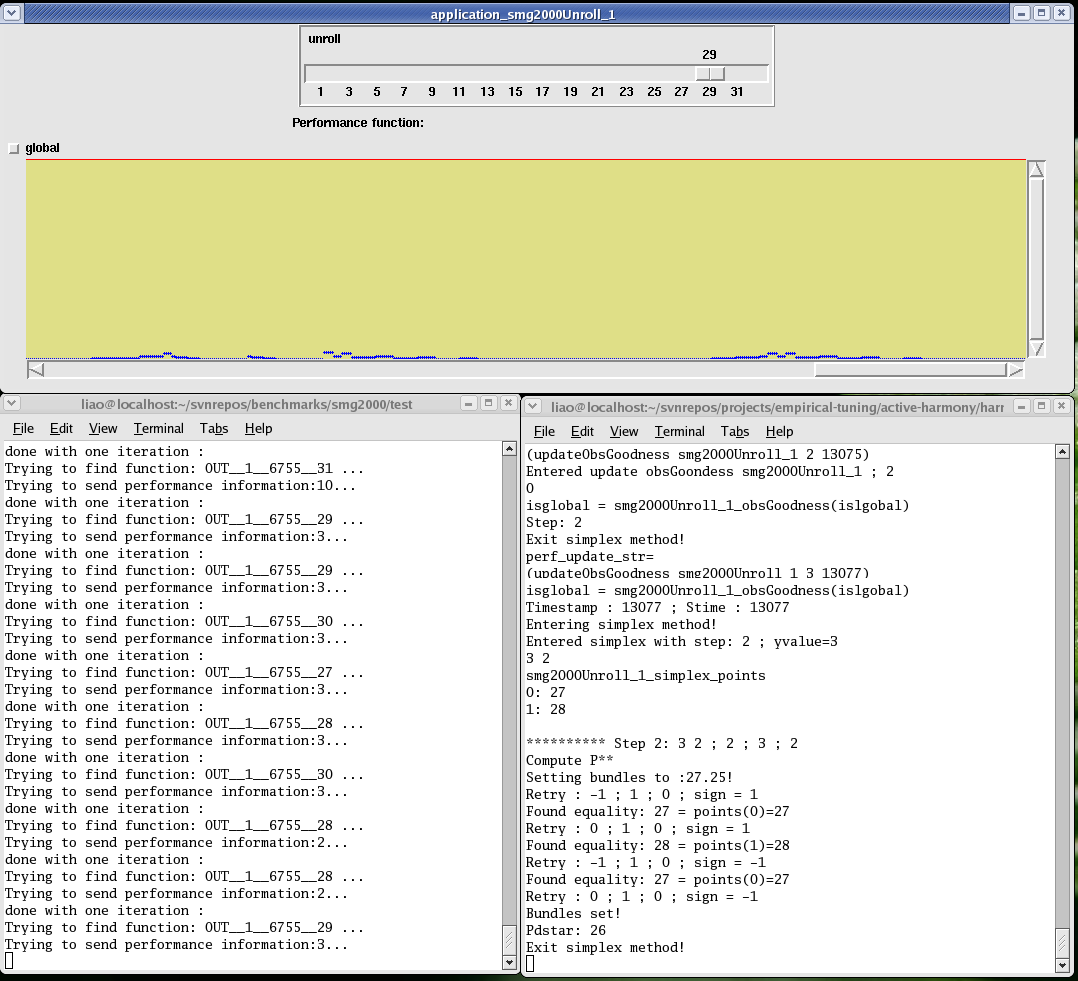
\includegraphics[width=0.8\textwidth]{activeHarmony2.png}
        \caption{Searching using Active Harmony}
        \label{fig:activeHarmony2}
\end{figure}

We have found that online/runtime search engines like the Active Harmony can be extremely expensive if the tuned kernel are invoked thousands of times. 
For SMG2000, it took hours to finish the tuning using a 120x120x120 input data set.
The major reason is that for each call of the kernel, a bidirectional communication between the client application and the server has to be finished. 
Another reason is that the current tuning process is embedded into the thousands of calls of the kernel so that points are always evaluated even when some of them have already been evaluated before. 


